\documentclass[a4paper, fleqn]{article}
\usepackage[margin=0.5in]{geometry} % page layout
\usepackage{amsmath,amssymb,amsthm} % maths packages
\usepackage{tikz-cd} % commutative diagrams
\usepackage[colorlinks, linkcolor=black, urlcolor=black, citecolor=black]{hyperref} % hyperreferences with black links
\usepackage{graphicx} % graphics
\usepackage{multicol} % multiple columns
\usepackage[none]{hyphenat}  % Prevent hyphenation
\usepackage{microtype} % Improves spacing

\setlength{\parindent}{0pt} % Set the indent for new paragraphs to 0
\setlength{\mathindent}{0pt} % Set the indent for equations to 0

\tolerance=1000
\emergencystretch=\maxdimen
\hyphenpenalty=1000
\hbadness=10000

% Set up Diagram Paths
\graphicspath{{../Graphs}}

% Theorem environments
\theoremstyle{plain}
\newtheorem{theorem}{Theorem}[section]
\newtheorem{proposition}[theorem]{Proposition}
\newtheorem{lemma}[theorem]{Lemma}
\newtheorem{corollary}[theorem]{Corollary}
\newtheorem{claim}[theorem]{Claim}
\newtheorem{conjecture}{Conjecture}
\theoremstyle{definition}
\newtheorem{remark}[theorem]{Remark}
\newtheorem{definition}[theorem]{Definition}
\newtheorem{example}[theorem]{Example}

\RequirePackage{etoolbox}
\AtEndEnvironment{remark}{\hfill$\lozenge$}
\AtEndEnvironment{example}{\hfill$\lozenge$}

% Auxiliary commands
\DeclareMathSymbol{:}{\mathpunct}{operators}{"3A}%semicolon spaces
\RequirePackage{xspace}
\def\mat#1{\ensuremath{#1}\xspace}
\def\dmat#1#2{\gdef#1{\mat{#2}}}
\def\csdmat#1#2{\csdef{#1}{\mat{#2}}}

% Operators. Usage: \GL
\def\oper#1{\csdmat{#1}{\operatorname{#1}}}
\forcsvlist\oper{GL,SL,deg,Hom,End,Vect,Mod,Rep,Ker,Im,Id}

% Mathbb Letters. Usage: \bA
\def\defbb#1{\csdmat{b#1}{\mathbb{#1}}}
\forcsvlist\defbb{A,B,C,D,E,F,G,H,I,J,K,L,M,N,O,P,Q,R,S,T,U,V,W,X,Y,Z}
\RequirePackage{bbm}
\dmat\bk{\mathbbm k}

% Mathcal Letters. Usage: \cA
\def\defcal#1{\csdmat{c#1}{\mathcal{#1}}}
\forcsvlist\defcal{A,B,C,D,E,F,G,H,I,J,K,L,M,N,O,P,Q,R,S,T,U,V,W,X,Y,Z}

% Greek letters
\dmat\al\alpha
\dmat\be\beta
\dmat\ga\gamma
\dmat\de\delta
\dmat\la\lambda
\dmat\ta\tau
\dmat\hi\chi
\dmat\eps\varepsilon
\dmat\vi\phi
\dmat\te\theta
\dmat\ksi\xi
\dmat\si\sigma
\dmat\om\omega
\dmat\Ga\Gamma
\dmat\La\Lambda

% Structures
\def\set#1{\left\{#1\right\}}
\def\sets#1#2{\left\{\left.#1\ \right\vert#2\right\}}
\def\rbr#1{\left(#1\right)}
\def\ang#1{\left\langle#1\right\rangle}
\def\n#1{\left\lvert#1\right\rvert}
\def\nn#1{\left\lVert#1\right\rVert}
\def\eq#1{\begin{equation}#1\end{equation}}
\def\ov#1#2{{\substack{#1\\#2}}} % #1 over #2

% Symbols
\def\mto{\mapsto}
\def\emb{\hookrightarrow}
\def\es{\emptyset}
\def\bs{\backslash}
 % file with useful abbreviations

\begin{document}

\title{\bf\Huge Concerning the Stability \\ of \\ Complex Time Steppers}
\author{\Large Cian J. Duggan}
\date{\today}

\maketitle
\thispagestyle{empty}
\newpage

\tableofcontents
\thispagestyle{empty}
\newpage
\setcounter{page}{1}

\newpage
\section{Introduction}
\par A paper by Lloyd N. Trefethen~\cite{trefethen_definition} offers two definitions of numerical analysis:
\begin{quote}
    \textit{The study of rounding errors.}
\end{quote}
\begin{quote}
    \textit{The study of algorithms for the problems of continuous mathematics.}
\end{quote}

\par Trefethen argues that the first definition, though an accurate summation of the field's history, does not serve to entice the curious to explore the field. He proposes the second as a more compelling definition, one that emphasises the field's role in solving real-world problems, and inspires curiosity.

\par He offers an optimistic view of the field, one that is not bogged down by the minutiae of rounding errors, but rather one that is focused on the algorithms that make numerical analysis possible. More to ground, the majoirity of numerical analysis is concerned with the speed of convergence and minimization of error.

Through my work on this paper, I have honed my own definition:
\begin{quote}
	\textit{Numerical analysis is the field which attempts to straddle the gaps between the discrete and the continuous.}
\end{quote}

In this paper we will take a look at the stability of various numerical methods when applied to problems of differential calculus.\\
In particular, we wish to:
\begin{itemize}
	\item[$\cdot$] Introduce key terminology and concepts in the field of numerical analysis.
	\item[$\cdot$] Establish the Exponential Decay Problem as the toy problem for analysis.
	\item[$\cdot$] Define stability, and its associated concepts, in the context of numerical analysis.
	\item[$\cdot$] Establish the concept of Complex time steps for numerical methods.
	\item[$\cdot$] Develop a framework for the analysis of the stability of numerical methods.
	\item[$\cdot$] Apply this framework to particular numerical methods.
	\item[$\cdot$] Expand upon the results of this to contrast the stability regions for Real and Complex time steps.
	\item[$\cdot$] MORE?
\end{itemize}

\newpage
\section{Definitions and Concepts}

\subsection{Numerical Methods}
\par \term{Numerical methods} are techniques used to approximate solutions to problems that cannot be solved exactly.\\
Numerical methods are prevalent when working with problems of differential calculus in a computational context, where many problems do not have closed-form solutions.\\
A numerical method can be interpreted as an alogorithm; a series of steps that can be followed to approximate a solution.\\
Many numerical methods exist, each with their own properties and tradeoffs.\\
In this respect, different methods may be more or less suitable for different problems.\\
Core to understanding which to use for a particular problem are the concepts of \term{error} and \term{stability}.\\
Before discussing these properties, however, we must understand how a numerical method works.\\
The basis of many numerical methods is the concept of a \term{time step}.

\subsection{Time Steps}
Let's take a step back to when we first studied derivatives.\\
\term{Newton's Difference Quotient} should be familiar: 
$f'(x) = \Lim{h \to 0} \frac{f(x+h) - f(x)}{h}$

\par Viewing Newton's Difference Quotient in the context of numerical methods, we call $h$ a \term{time step}.\\
Due to computational constraints, we cannot take $h$ to be infinitesimal. (A computer's memory is as small as it is big)\\
Instead, we take $h$ to be a small, finite number.\\
This defines the concept of a \term{step size}.\\

\par For numerical methods, we use $y(t)$ to denote the solution to a differential equation at time $t$.\\
We approximate $y'(t)$ by $\frac{y(t+h) - y(t)}{h}$ using Newton's Difference Quotient.\\
Note this is an approximation because we have dropped the limit; $h$ is not infinitesimal.\\
This gives $y(t + h) \approx y(t) + h y'(t)$; a first-order approximation of $y$ a small time step $h$ in the future.\\
For a numerical method we say $y(t + h) = y(t) + h y'(t)$ 

\subsection{Error}
\par In numerical analysis, \term{error} is the difference between the numerical solution and the exact solution to a problem.\\
Error can be caused by many factors, such as the choice of numerical method, the choice of time step, or the precision of the computer.\\
Error can be classified into two categories: truncation error and rounding error.\\
\term{Truncation Error} is the error introduced by approximating a problem, such as using a finite time step.\\
\term{Rounding Error} is the error introduced by the finite precision of a computer.\\
Error is a crucial concept in numerical analysis, as it determines the accuracy of a numerical method.\\
Any error mentioned in this document refers to the truncation error; we won't be looking at how comupters run these calculations and the rounding errors that come with it.

\subsection{Stability}
\par In numerical analysis, a method is said to be \term{stable} if small deviations in the input do not lead to large perturbtions in the output.
In the context of differential equations, a method is said to be stable if the solution does not grow to be unbounded as the number of time steps increases. (This, of course, only applies if the exact solution is bounded. We will restrict ourselves to this with our analysis.)

\par When solving differential equations numerically, the choice of time step is crucial.
If the step size is too large, the solution may become unstable; the numerical solution will diverge from the analytic solution in proportion with the number of steps.
If the step size is too small, the solution may be accurate and stable, but the computation may be too slow.

\par The tradeoff between error, stability and compute is a common theme in numerical analysis.\\
The sweet spot for maximal efficiency depends entirely on the choice of numerical method.\\
This marks the core motivation for this report; solidifying an understanding to better inform the choice of method and step size for a given problem.

%\subsection{Complex-Variable Method}
%Take a function $f: \bR \longrightarrow \bR,\; x \longmapsto f(x)$.\\
%Let $f$ be \term{holomorphic} on its domain: $f$ is complex differentiable in a neighbourhood of any $x \in \bR$.\\
%$\forall x$, $f$ is complex differentiable on $B_{\beta}(x) = \{z \in \bC \,|\, |z|-|x| < \beta_{_{\text{small}}}\}$ for some $\beta_{_{\text{small}}} > 0$.\\
%In this case, we get the following fact:\\
%\[f'(x) = \frac{Im\big(f(x+ih)\big)}{h} + O(h^2), \quad \text{where}\; h \in \bR \;\text{and}\; h \neq 0\]\\

%\par Combining this with the first order approximation above, we get $y(t + \Delta_t) \approx y(t) + Im\big(y(t+i\Delta_t)\big)$.

%TODO: Flesh this out more!

\newpage
\section{Stability Analysis}

\subsection{Introduction}
In this section we will lay out a framework for analysing the stability of a numerical method dependant on time steps.
To begin, we will consider a simple toy problem to illustrate the concept of stability.
We will introduce the concept of the stability function and show how it can be used to analyse the stability of a numerical method.
Finally, we will extend this framework to view the stability of a numerical method as a function of complex time steps.



\subsection{Exponential Decay Problem}

\par We would like a simple toy problem on which we can build a framework for the analysis of the stability of a numerical method.\\
A common example across numerical analysis is the ODE exponential decay problem: 
\[y'(t) = \lambda y(t) \quad \text{with} \quad y(0) = 1 \;\text{and}\; Re(\lambda) < 0\]
Where the constant $\lambda \in \bC$ can be interpreted as the decay rate of the solution.\\
This has the exact solution $y(t) = e^{\lambda t}$.\\

\subsubsection{Proponents of the Exponential Decay Problem}
\par There are a few pros to this choice of problem:
\begin{itemize}
    \item The exact solution is known and easily computed; it can be used to evaluate a numerical solution.
    \item The solution is a straigtforward and well understood function.\\
    	  This simplicity allows us to focus on the numerical method.
    \item The problem is linear in $y(t)$, making the problem simple to work with.\\
    	  Again, our focus can stay on the numerical method.
    \item The graph of the exact solution is easy to visualise; the more chaotic outputs of the numerical methods can be compared to the smooth curve of the exact solution easily.
    \item Exponential decay is a model for many physical processes, including radioactive decay, population decay, and capacitor discharge.\\
    	  This means readers from many different disciplines already posses an intuition for the problem.
    \item The problem is simple to generalise to complex numbers, allowing us to explore the stability of numerical methods in the complex plane.
    \item Stiffness. WRITE MORE
    \item Generalisation. WRITE MORE
\end{itemize}

\subsubsection{Additional Details}
\begin{multicols}{2}
The Taylor series for the exact solution is 
\[y(t) = \sum\limits_{n=0}^{\infty} \frac{{(t)}^n}{n!}\]

The solution decays to zero as $t \rightarrow \infty$ when $Re(\lambda) < 0$.\\

\par Normally, when using the exponential decay problem in a numerical analysis context, we would allow $\lambda \in \bC$ with $Re(\lambda)<0$.\\
However, for the purposes of this paper, we will restrict $\lambda$ to $\bR$ as we will be looking at $h \in \bC$ and we don't want to overcomplicate things.\\
Unless otherwise mentioned, we will assume that $\lambda \in \bR^{-}$ for the rest of this paper.\\

\par $\phi(t, y) = y'(t) = \lambda y(t)$ is linear in $y(t)$\\

\columnbreak{}
\hspace*{0.75cm}
A lot of the findings in this paper will be represented\\
\hspace*{0.75cm}
graphically.\\
\hspace*{0.75cm}
Let's start with the most basic.\\
\par \hspace*{0.75cm}
Here's a graph of the exact solution for the\\ 
\hspace*{0.75cm}
exponential decay problem with $\lambda = -1$:
\begin{center}
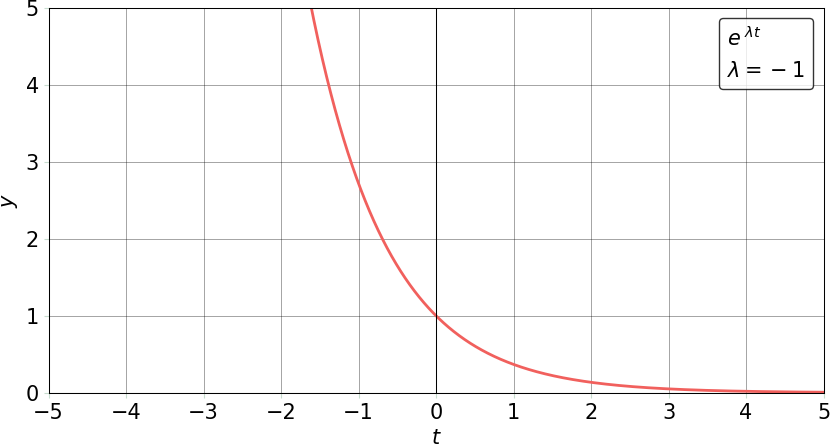
\includegraphics[width=0.4\textwidth]{Exponential Decay/Exact with -1.png}
\end{center}
\end{multicols}

\newpage
\subsection{Numerical Method: Forward Euler}

\par We will now consider a simple numerical method applied to the exponential decay problem.
The Forward Euler method is a first-order numerical method for solving ODEs with a given initial condition.
Its algorithm can be defined as follows:
\[ y(t_{j+1}) = y(t_j) + h y'(t_j) \qquad \text{Or equivalently:} \qquad y_{j+1} = y_j + h \phi(t_j, y_j)\]
Where $h$ is the time step and $y_j$ is the numerical solution at time $t_j$.

\par For the exponential decay problem, the Forward Euler method can be written as:
\[ y_{j+1} = y_j + h \lambda y_j \quad \text{where} \quad y_0 = 1\]
This gives us the following algorithm:
\[ y_{j+1} = (1 + h \lambda) y_j\]
This gives an approximation of the exact solution at time $t_j$ as follows:
\[ y_{j} \approx {(1 + h \lambda)}^j y_0\]

\par We can see that the Forward Euler method is stable if $|1 + h \lambda| < 1$; both the exact solution and our approximation will decay to zero as $t \rightarrow \infty$.
The stability is dependent on the time step $h$ and the value of $\lambda$.
We can write this as $s(\lambda, h) = 1 + h \lambda$.
By analysing $s$ for different values of $\lambda$ and $h$, we can infer the stability of the Forward Euler method for the exponential decay problem.
We call $s$ the \term{stability function} of the Forward Euler method.



\subsection{The Stability Function and corresponding Stability Region}
\par By the same methodology, we can define the stability function for any numerical method:\\
Write the algorithm in the form $y_{j+1} = s(\lambda, h) y_{j}$.\\
$s(\lambda, h)$ is the \term{stability function} of the numerical method with a time step $h$.\\
\textbf{Note:} This is equivalent to $y_{j} = {s(\lambda,h)}^{j} y_0$

\par The \term{stability region} of a numerical method is the set $S = \Big\{ (\lambda, h) \;\Big|\; |s(\lambda, h)| < 1\Big\}$\\
This follows from the definition of stability for our exponential decay problem; a method is stable if the numerical solution decays to zero as $t \rightarrow \infty$.\\
Clearly, $y_{j} = {s(\lambda,h)}^{j} y_0$ will decay to zero as $j \rightarrow \infty$ if $|s(\lambda, h)| < 1$.

\subsubsection{Stability Region for Euler's Forward Method}
\begin{multicols}{2}
\vspace*{\fill}

Euler's Forward Method has the stability function
\[s(\lambda, h) = 1 + \lh\]
The corresponding stability region is 
\[S = \Big\{ (\lambda, h) \;\Big|\; |1 + \lh| < 1\Big\}\]
We can see this region plotted in red on the right; an open unit circle centred at $-1$.\\
For a given $\lambda \in \bC$, the method is stable for any step-size $h \in \bR$ such that $|1 + \lh| < 1$.\\
Expanding $\lambda = a + bi$, we get the restriction
\[|1 + (a + bi)h| < 1 \quad \implies \quad a^2h^2 + 2ah + b^2h^2 < 0\]
As $a, b$ and $h \in \bR$, $(a^2 +b^2)h^2 > 0$\\
$\implies 2ah < 0$ with $|2ah| > (a^2 + b^2)h^2$

\vspace*{\fill}
\columnbreak{}
\begin{center}
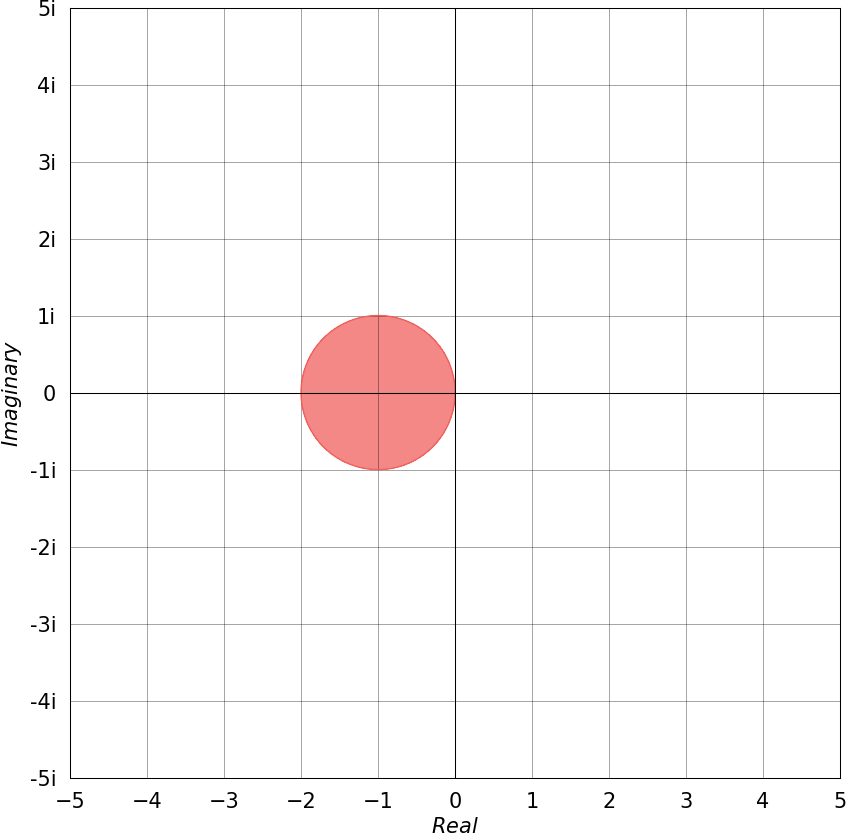
\includegraphics[width=0.49\textwidth]{Stability Regions/Graphs/Real 1-Step/Euler's Forward.png}
\end{center}
\end{multicols}

\subsubsection{Stability Region for Euler's Backward Method}
\begin{multicols}{2}
\begin{center}
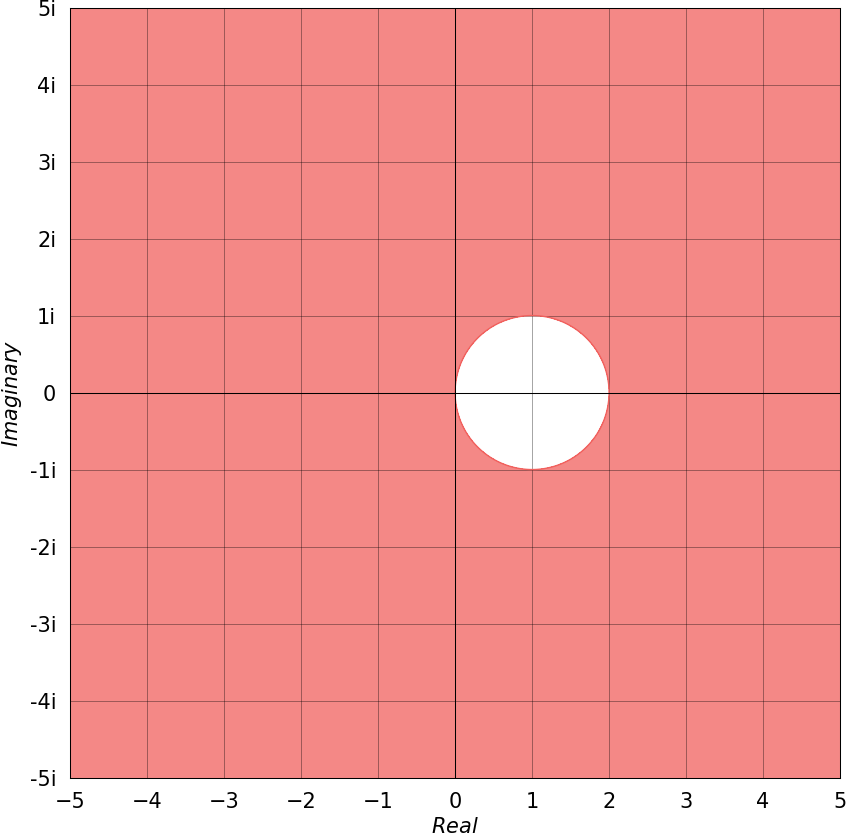
\includegraphics[width=0.49\textwidth]{Stability Regions/Graphs/Real 1-Step/Euler's Backward.png}
\end{center}
\columnbreak{}
\vspace*{\fill}

Euler's Backward Method can be written as
\[y_{j+1} = y_j + h.\phi(t_{j+1}, y_{j+1})\]
\[\implies y_{j+1} = y_j + h(\lambda y_{j+1}) \implies y_{j+1} = \frac{1}{1 - \lh}y_j\]
Thus, the stability function is
\[s(\lambda, h) = \frac{1}{1 - \lh}\]
The corresponding stability region is
\[S = \Big\{ (\lambda, h) \;\Big|\; \left|\frac{1}{1 - \lh}\right| < 1\Big\}\]
This is plotted in red on the left; the region outside a unit circle centred at $1$.\\
The white region of instability is exactly the stability region for Euler's Forward Method, flipped about Imaginary axis.\\
\vspace*{\fill}
\end{multicols}

\subsubsection{Stability Region for Runge-Kutta 4}
\begin{multicols}{2}
\vspace*{\fill}

Runge-Kutta 4 can be written as
\[y_{j+1} = y_j + \frac{h}{6}(k_1 + 2k_2 + 2k_3 + k_4)\]
Where
\begin{flalign*}
	k_1 &= \phi(t_j, y_j) \quad &k_2 = \phi(t_j + \frac{h}{2}, y_j + \frac{h}{2}k_1) && \\
	k_3 &= \phi(t_j + \frac{h}{2}, y_j + \frac{h}{2}k_2) \quad &k_4 = \phi(t_j + h, y_j + hk_3) &&
\end{flalign*}
For the Exponential Decay Problem, we get
\[y_{j+1} = (1 + \lh + \frac{{(\lh)}^2}{2} + \frac{{(\lh)}^3}{6} + \frac{{(\lh)}^4}{24})y_j\]
The stability function is $s(\lambda, h) = \sum\limits_{m=0}^{4}\frac{{(\lh)}^m}{m!}$\\
The corresponding stability region is
\[S = \Big\{ (\lambda, h) \;\Big|\; \left|\sum\limits_{m=0}^{4}\frac{{(\lh)}^m}{m!}\right| < 1\Big\}\]

\vspace*{\fill}
\columnbreak{}
\begin{center}
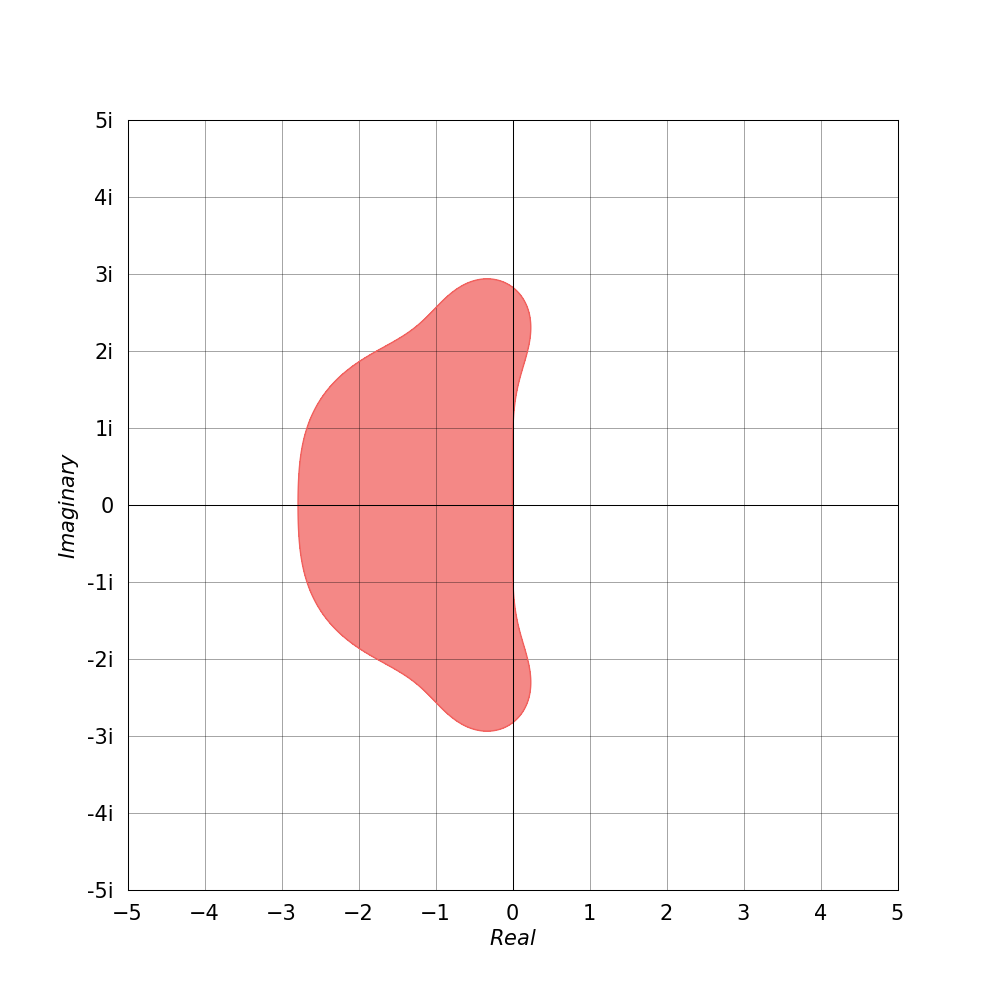
\includegraphics[width=0.49\textwidth]{Stability Regions/Graphs/Real 1-Step/Runge-Kutta 4.png}
\end{center}
\end{multicols}

\subsection{Interpretation of Stability Regions}
\par In the first graph, shaded in grey, is the region of stability for Runge-Kutta 4.\\
This region is the set of $\lh$ values for which the method is stable.\\

\par In all other graphs, in black, is a plot of the exact solution to the Exponential Decay Problem for a given $\lambda$.
For this curve to appear smooth, a step-size in t of $h = \frac{1}{1000}$ was used.\\

\par As we have fixed $h$, the stability region gives the set of values $\frac{\lambda}{1000}$ for which the method is stable.\\
From this we can derive stable $\lambda$ values.

\par Highlighted on the left are $n$ coloured points, representing $n$ different values of $\frac{\lambda}{1000}$.
The green point is $-1$, and sits inside the stability region.
This tells us that the method is stable for $\lambda = -1000$.\\
We can see this on the right, as the green curve of RK4 with $\lambda = -1000$ decays to zero and closely follows the exact solution in black.\\

MORE DETAIL HERE\\


\subsection{Numerical Method: 2-step Abysmal Kramer-Butler Method}

\par This method was designed to be unstable for the sake of demonstration.\\
The algorithm is as follows:
\[y_{j+1} = y_{j-1} + h(4\phi(t_j,y_j)-2\phi(t_{j-1},y_{j-1}))\]
As we know the exact solution to our Exponential Decay problem is $y(t) = e^{\lambda t}$, we know $\phi(t,y) = \lambda y$.\\
This gives:\\
\[y_{j+1} = y_{j-1} + h(4\lambda y_j - 2\lambda y_{j-1})\]
Simplified:\\
\[y_{j+1} = 4\lh y_j + (1-2\lh) y_{j-1}\]
%FURTHER DERIVATION ON WHITEBOARD - Aim: Get method in terms of $y_{j}$, $y_1$ and $y_0$ only.\\

\newpage
\section{Complex Time-Steps}
So far, we have restricted ourselves to time-steps in the real domain.\\
It has often proven useful to extend the analysis of a problem to the complex domain.\\
Motivated by a paper by \textit{George, Yung and Mangan}\cite{walking_into_the_complex_domain}, we will have a look at the stability of numerical methods when the chosen time-step is complex.\\
They state: \begin{quote} \textit {Most numerical methods for time integration use real time steps. Complex time steps provide an additional degree of freedom, as we can select the magnitude of the step in both the real and imaginary directions. By time stepping along specific paths in the complex plane, integrators can gain higher orders of accuracy or achieve expanded stability regions.}\end{quote}

\subsection{Complex 2-Step}
\begin{multicols}{2}
\par We want to take an overall step of size $\lh \in \bR$ comprised of two steps $z_1, z_2 \in \bC$ such that $z_1 + z_2 = \lh$.\\
We can set $z_1 = a + bi$ and $z_2 = \lh - a - bi$.\\
For analysing our numerical methods, we require a comparable implementation of the real step setup.\\

\par A real 2-step method where we take a step of size $\frac{\lh}{2}$ allows us to take two steps and go the same distance as the complex 2-step method.\\
We can write this real 2-step method as $y_{j+1} = {s(\lambda, \frac{h}{2})}^{2} y_j$.\\
\textbf{Note:} We can write this explicitly as 
\[y_{j+1} = s(\lambda, \frac{h}{2}) y_{j+\frac{1}{2}} = s(\lambda, \frac{h}{2}) s(\lambda, \frac{h}{2}) y_j\]

\par We can write the complex 2-step method as 
\[y_{j+1} = s(\lambda, z_1) s(\lambda, z_2) y_j\]
\textbf{Note:} We can write this explicitly as 
\[y_{j+1} = s(\lambda, z_1) y_{j+\frac{1}{2}} = s(\lambda, z_1) s(\lambda, z_2) y_j\]

\columnbreak{}
% Triangle diagram
\begin{tikzpicture}
	\draw[->] (0,0) -- (8,0) node[right] {$Re$};
	\draw[->] (0,0) -- (0,8) node[above] {$Im$};
	\draw[-, color=orange] (0,0) -- (5,7) node[midway, shift={(-0.2,0)}, left] {$z_1$};
	\draw[-, color=orange] (5,7) -- (7,0) node[midway, shift={(0.1,0)}, right] {$z_1 + z_2$};
	\draw[color=purple] (0,0) -- (7,0) node[midway, below] {$\lh$};
\end{tikzpicture}
\end{multicols}


\subsection{Complex Conjugate Pairs}
\begin{multicols}{2}
% Triangle diagram
\begin{tikzpicture}
	\draw[->] (0,0) -- (7,0) node[right] {$Re$};
	\draw[->] (0,0) -- (0,4.5) node[above] {$Im$};
	\draw[-, color=orange] (0,0) -- (3,3.5) node[midway, shift={(-0.2,0)}, left] {$z$};
	\draw[-, color=orange] (3,3.5) -- (6,0) node[midway, shift={(0.1,0)}, right] {$z + \bar{z}$};
	\draw[-, color=purple] (0,0) -- (3,0) node[midway, below] {$\frac{\lh}{2}$};
	\draw[-, color=purple] (3,0) -- (6,0) node[midway, below] {$\frac{\lh}{2}$};
	\draw[-, color=blue] (3,0) -- (3,3.5) node[midway, right] {$b$};
\end{tikzpicture}
\columnbreak{}
\par When we restrict the exponential decay problem by $\lambda \in \bR$, we also find that $s(\lambda, z_1) s(\lambda, z_2) \in \bR$\\
This is because any value attained by $e^{\lambda t}$ is real.\\
This restricts the values of $z_1$ and $z_2$, as any imaginary terms in $s(\lambda, z_1) s(\lambda, z_2)$ must cancel out.\\

\par One particularly simple family of such complex pairs is defined by setting $a = \frac{\lh}{2}$\\
This necessitates $z_2 = \bar{z_1}$\\
We will refer to this family as the \term{complex conjugate step pairs}.\\
\end{multicols}

\newpage
\subsection{Stability of 2-Step Methods for Complex Conjugate Step Pairs}
\par In this section we will compare the stability regions for the real and complex 2-step methods.\\
The real step size is given by $\frac{\lh}{2}$\\
The complex conjugate step pair is given by $z = \frac{\lh}{2} + bi$ and $\bar{z} = \frac{\lh}{2} - bi$\\
The plots in this section show the regions of stability $S = \{h : |s(\lambda, h)| \leq 1\}$ for the case where $b=a=\frac{\lh}{2}$\\
We will have a look at varying $b$ in a subsequent section.\\

\subsubsection{Euler's Forward 2-Step}
\begin{multicols}{2}
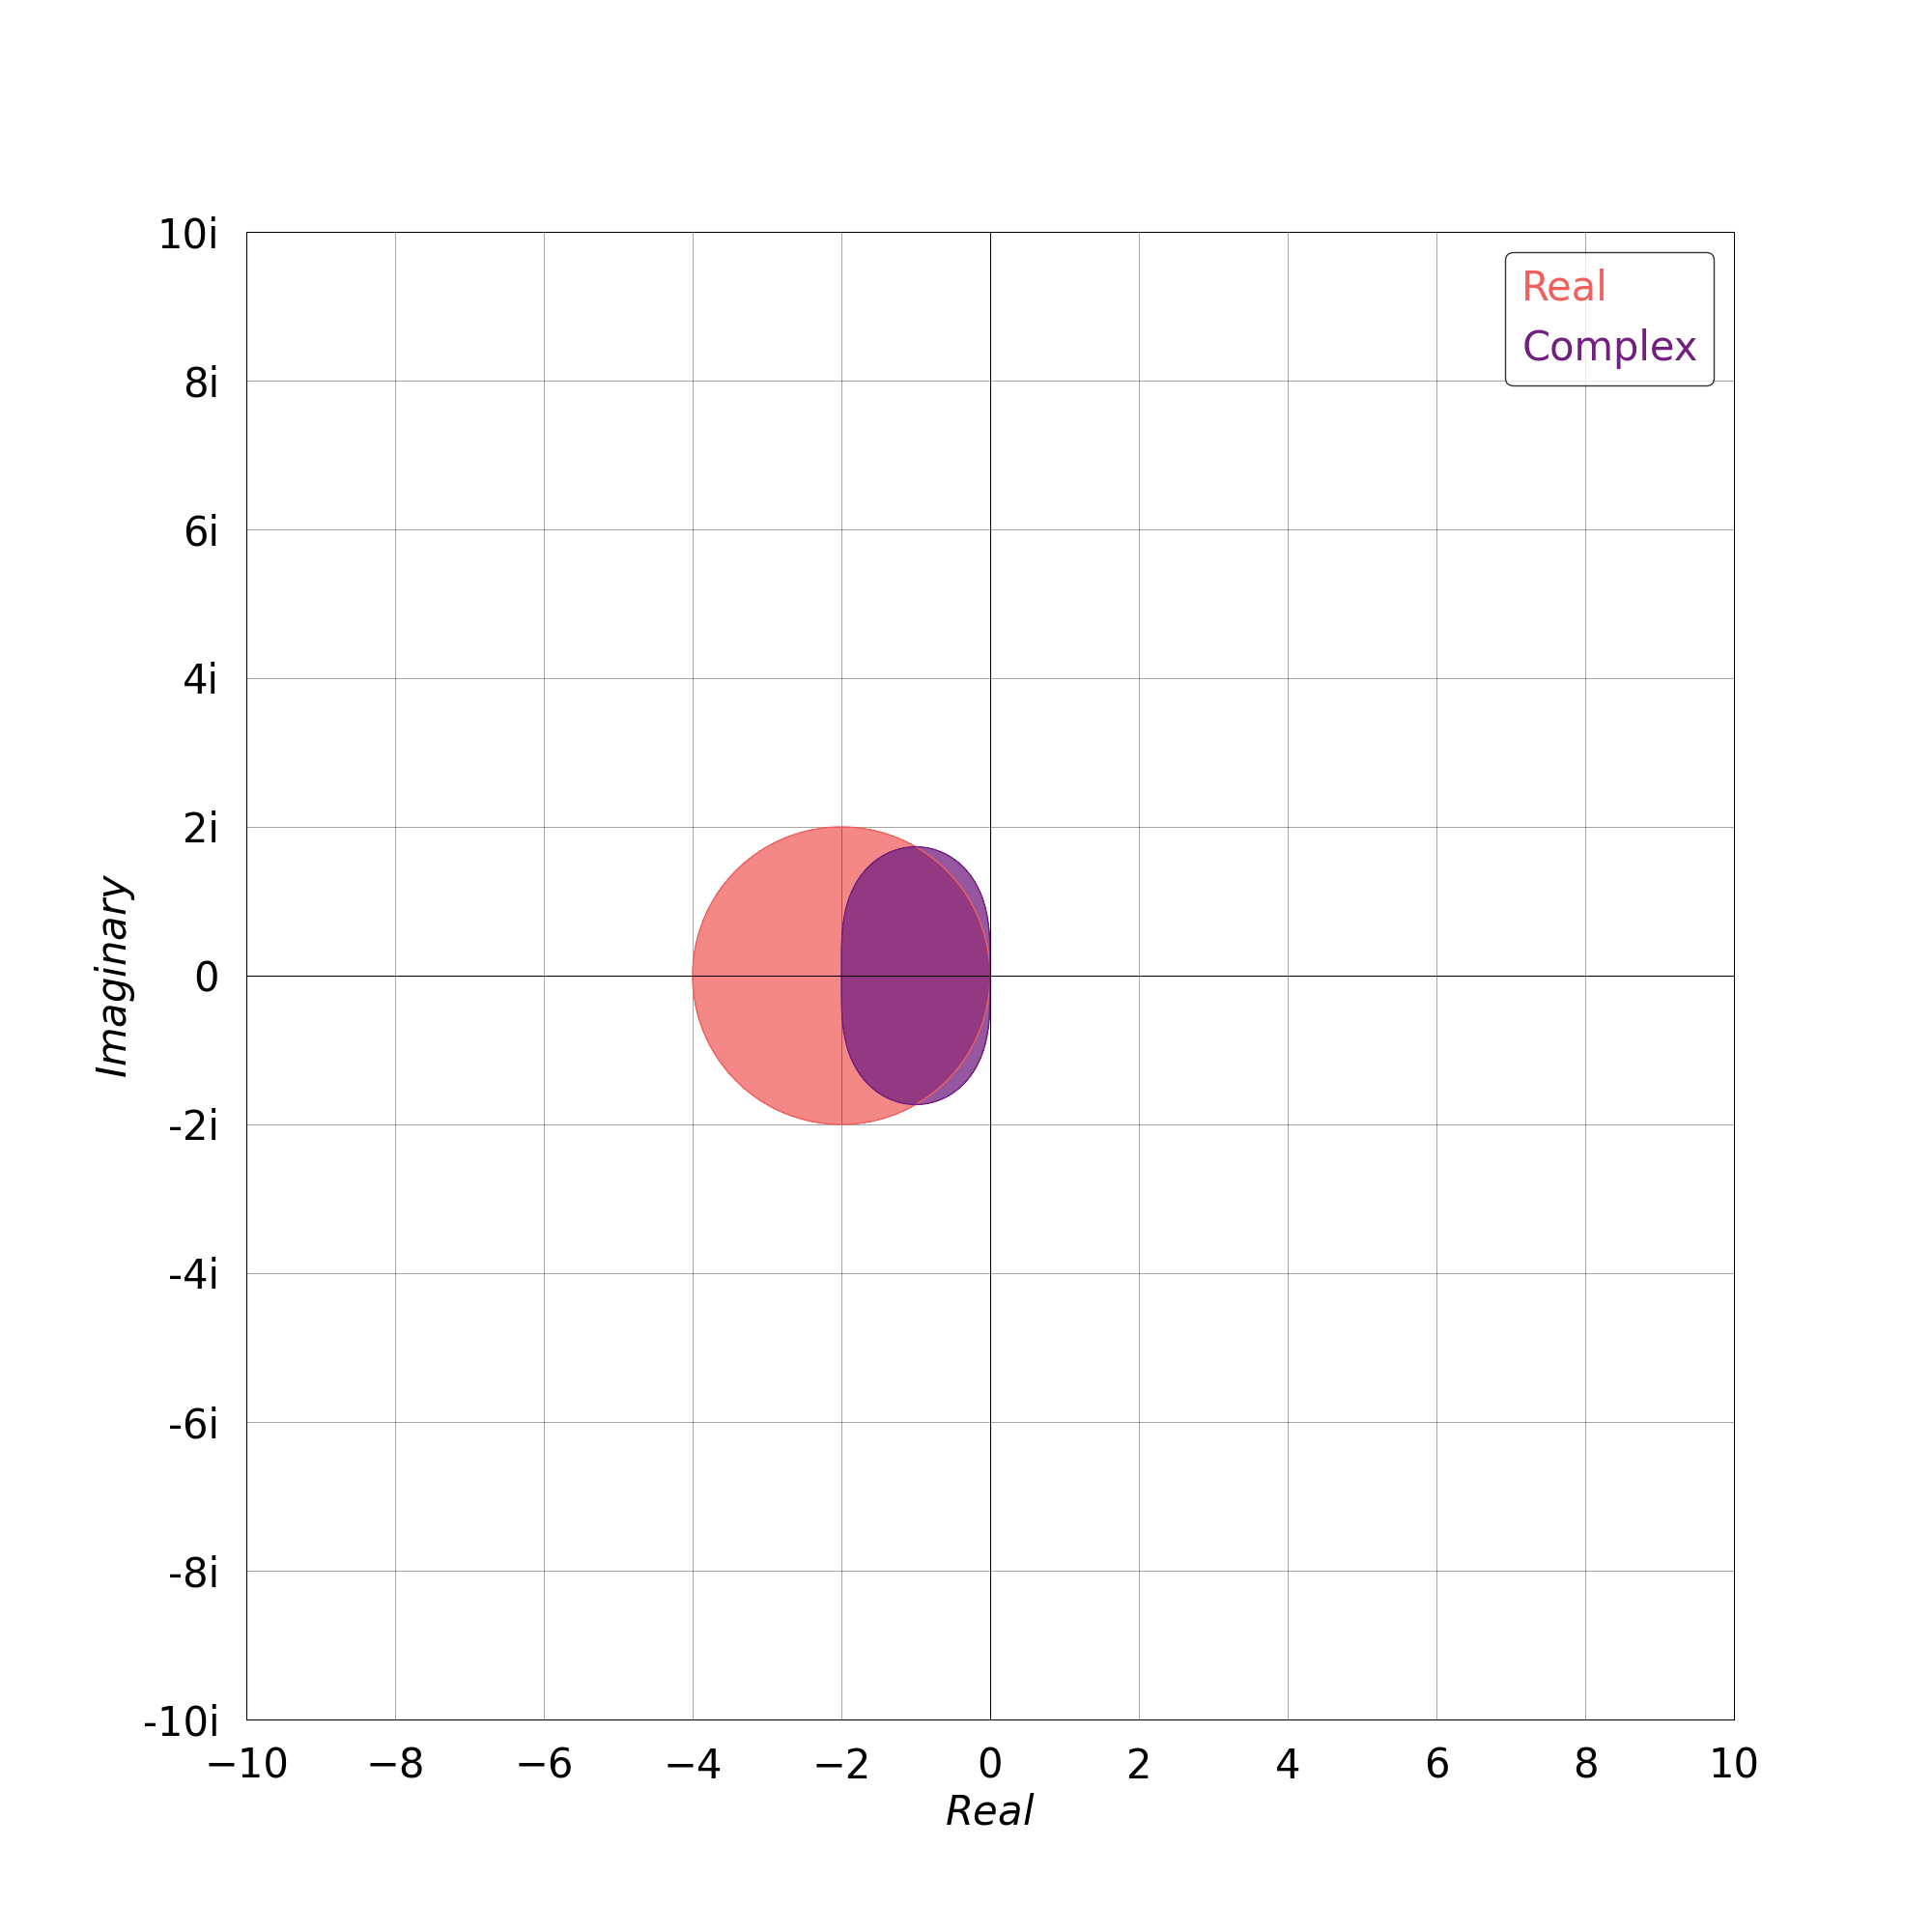
\includegraphics[height=8cm]{Stability Regions/Graphs/Real VS Complex Comparison/Euler's Forward.png}
\columnbreak{}

\textbf{Euler's Forward 2-Step $\bR$}
\begin{flalign*}
	y_{j+1} &= {\Big(1+ \frac{\lh}{2}\Big)}^2 y_j && \\
	\implies &s_{_{\bR}}(\lambda, h) = 1 + \lh + \frac{{(\lh)}^2}{4} &&
\end{flalign*}

\textbf{Euler's Forward 2-Step $\bC$}
\begin{flalign*}
	y_{j+1} &= \Big(1 + z\Big)\Big(1 + \bar{z}\Big) y_j && \\
	    &= \Big(1 + \frac{\lambda h}{2} + bi\Big)\Big(1 + \frac{\lambda h}{2} - bi\Big) y_j && \\
	    &= \bigg(\Big{(1 + \frac{\lambda h}{2}\Big)}^2 + b^2\bigg) y_j && \\
    \implies &s_{_{\mathbb{C}}}(\lambda, h) = 1 + \lambda h + \frac{{(\lambda h)}^2}{4} + b^2 && \\
    \implies &s_{_{\mathbb{C}}}(\lambda, h) = s_{_{\mathbb{R}}}(\lambda, h) + b^2 &&
\end{flalign*}

\vspace*{\fill}
\end{multicols}

\par As $b \in \bR$, $s_{_{\mathbb{C}}}(\lambda, h) \geq s_{_{\mathbb{R}}}(\lambda, h)$\\
This means the stability region for the complex 2-step method is smaller than that of the real 2-step method; there are less values of $\lh$ for which the complex 2-step method is stable.\\
$S_{_{\mathbb{C}}}$ is smaller than $S_{_{\mathbb{R}}}$\\
The diagram above illustrates the case where $b = a = \frac{\lh}{2}$\\

\par We can vary the $b$ value to see how the stability region changes.\\
This series of diagrams shows the stability regions for the complex 2-step method with varying $b$ values.\\

VIDEOS SHOW b BEING VARIED\\

\par We can do the same kind of analysis for other Numerical Methods.\\
Below are the same derivations and diagrams for the Backward Euler and Runge-Kutta 4 methods.\\

\subsubsection{Euler's Backward 2-Step}
\begin{multicols}{2}
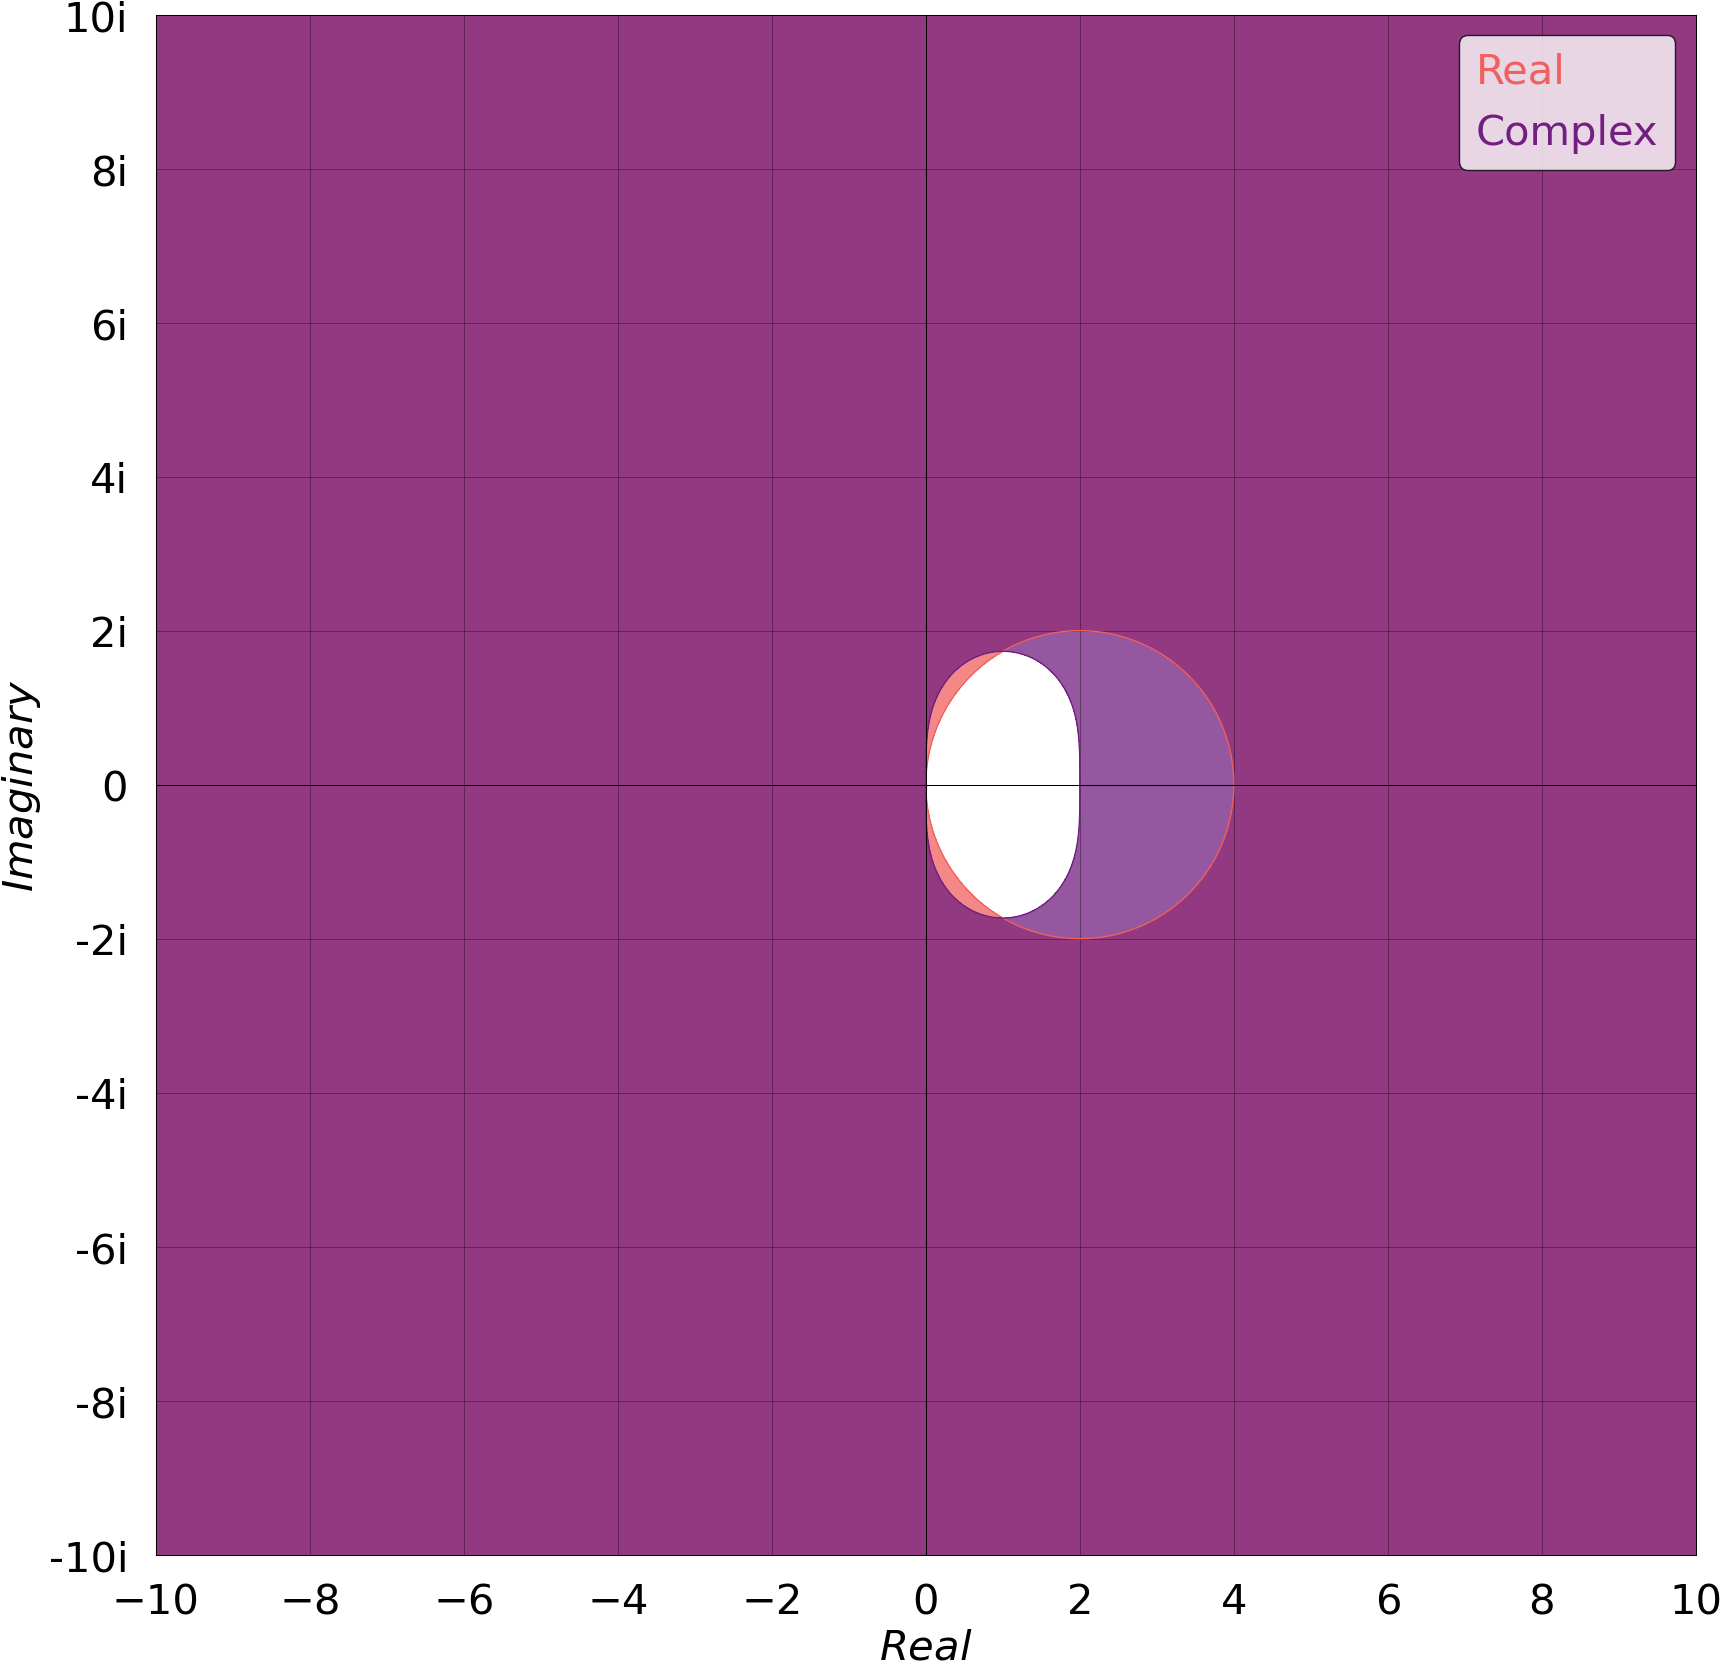
\includegraphics[height=8cm]{Stability Regions/Graphs/Real VS Complex Comparison/Euler's Backward.png}
\columnbreak{}

\textbf{Euler's Backward 2-Step $\bR$}
\begin{flalign*}
	y_{j+1} &= {\bigg(\frac{1}{1-\frac{\lh}{2}}\bigg)}^2 y_j && \\
	\implies & s_{\bR}(\lambda, h) = \frac{1}{1 - \lh + \frac{{(\lh)}^2}{4}} &&
\end{flalign*}

\textbf{Euler's Backward 2-Step $\bC$}
\begin{flalign*}
	y_{j+1} &= \bigg(\frac{1}{1-\frac{\lh}{2}+bi}\bigg)\bigg(\frac{1}{1-\frac{\lh}{2}-bi}\bigg)y_j && \\
    \implies &s_{\bC}(\lambda, h) = \frac{1}{1 - \lh + \frac{{(\lh)}^2}{4} + b^2} && \\
\end{flalign*}

\vspace*{\fill}
\end{multicols}

\par Again, $b \in \bR$, so this time, $s_{_{\mathbb{C}}}(\lambda, h) \leq s_{_{\mathbb{R}}}(\lambda, h) \implies S_{_{\mathbb{C}}}$ is larger than $S_{_{\mathbb{R}}}$\\

\subsubsection{Runge-Kutta 4 2-Step}
\begin{multicols}{2}
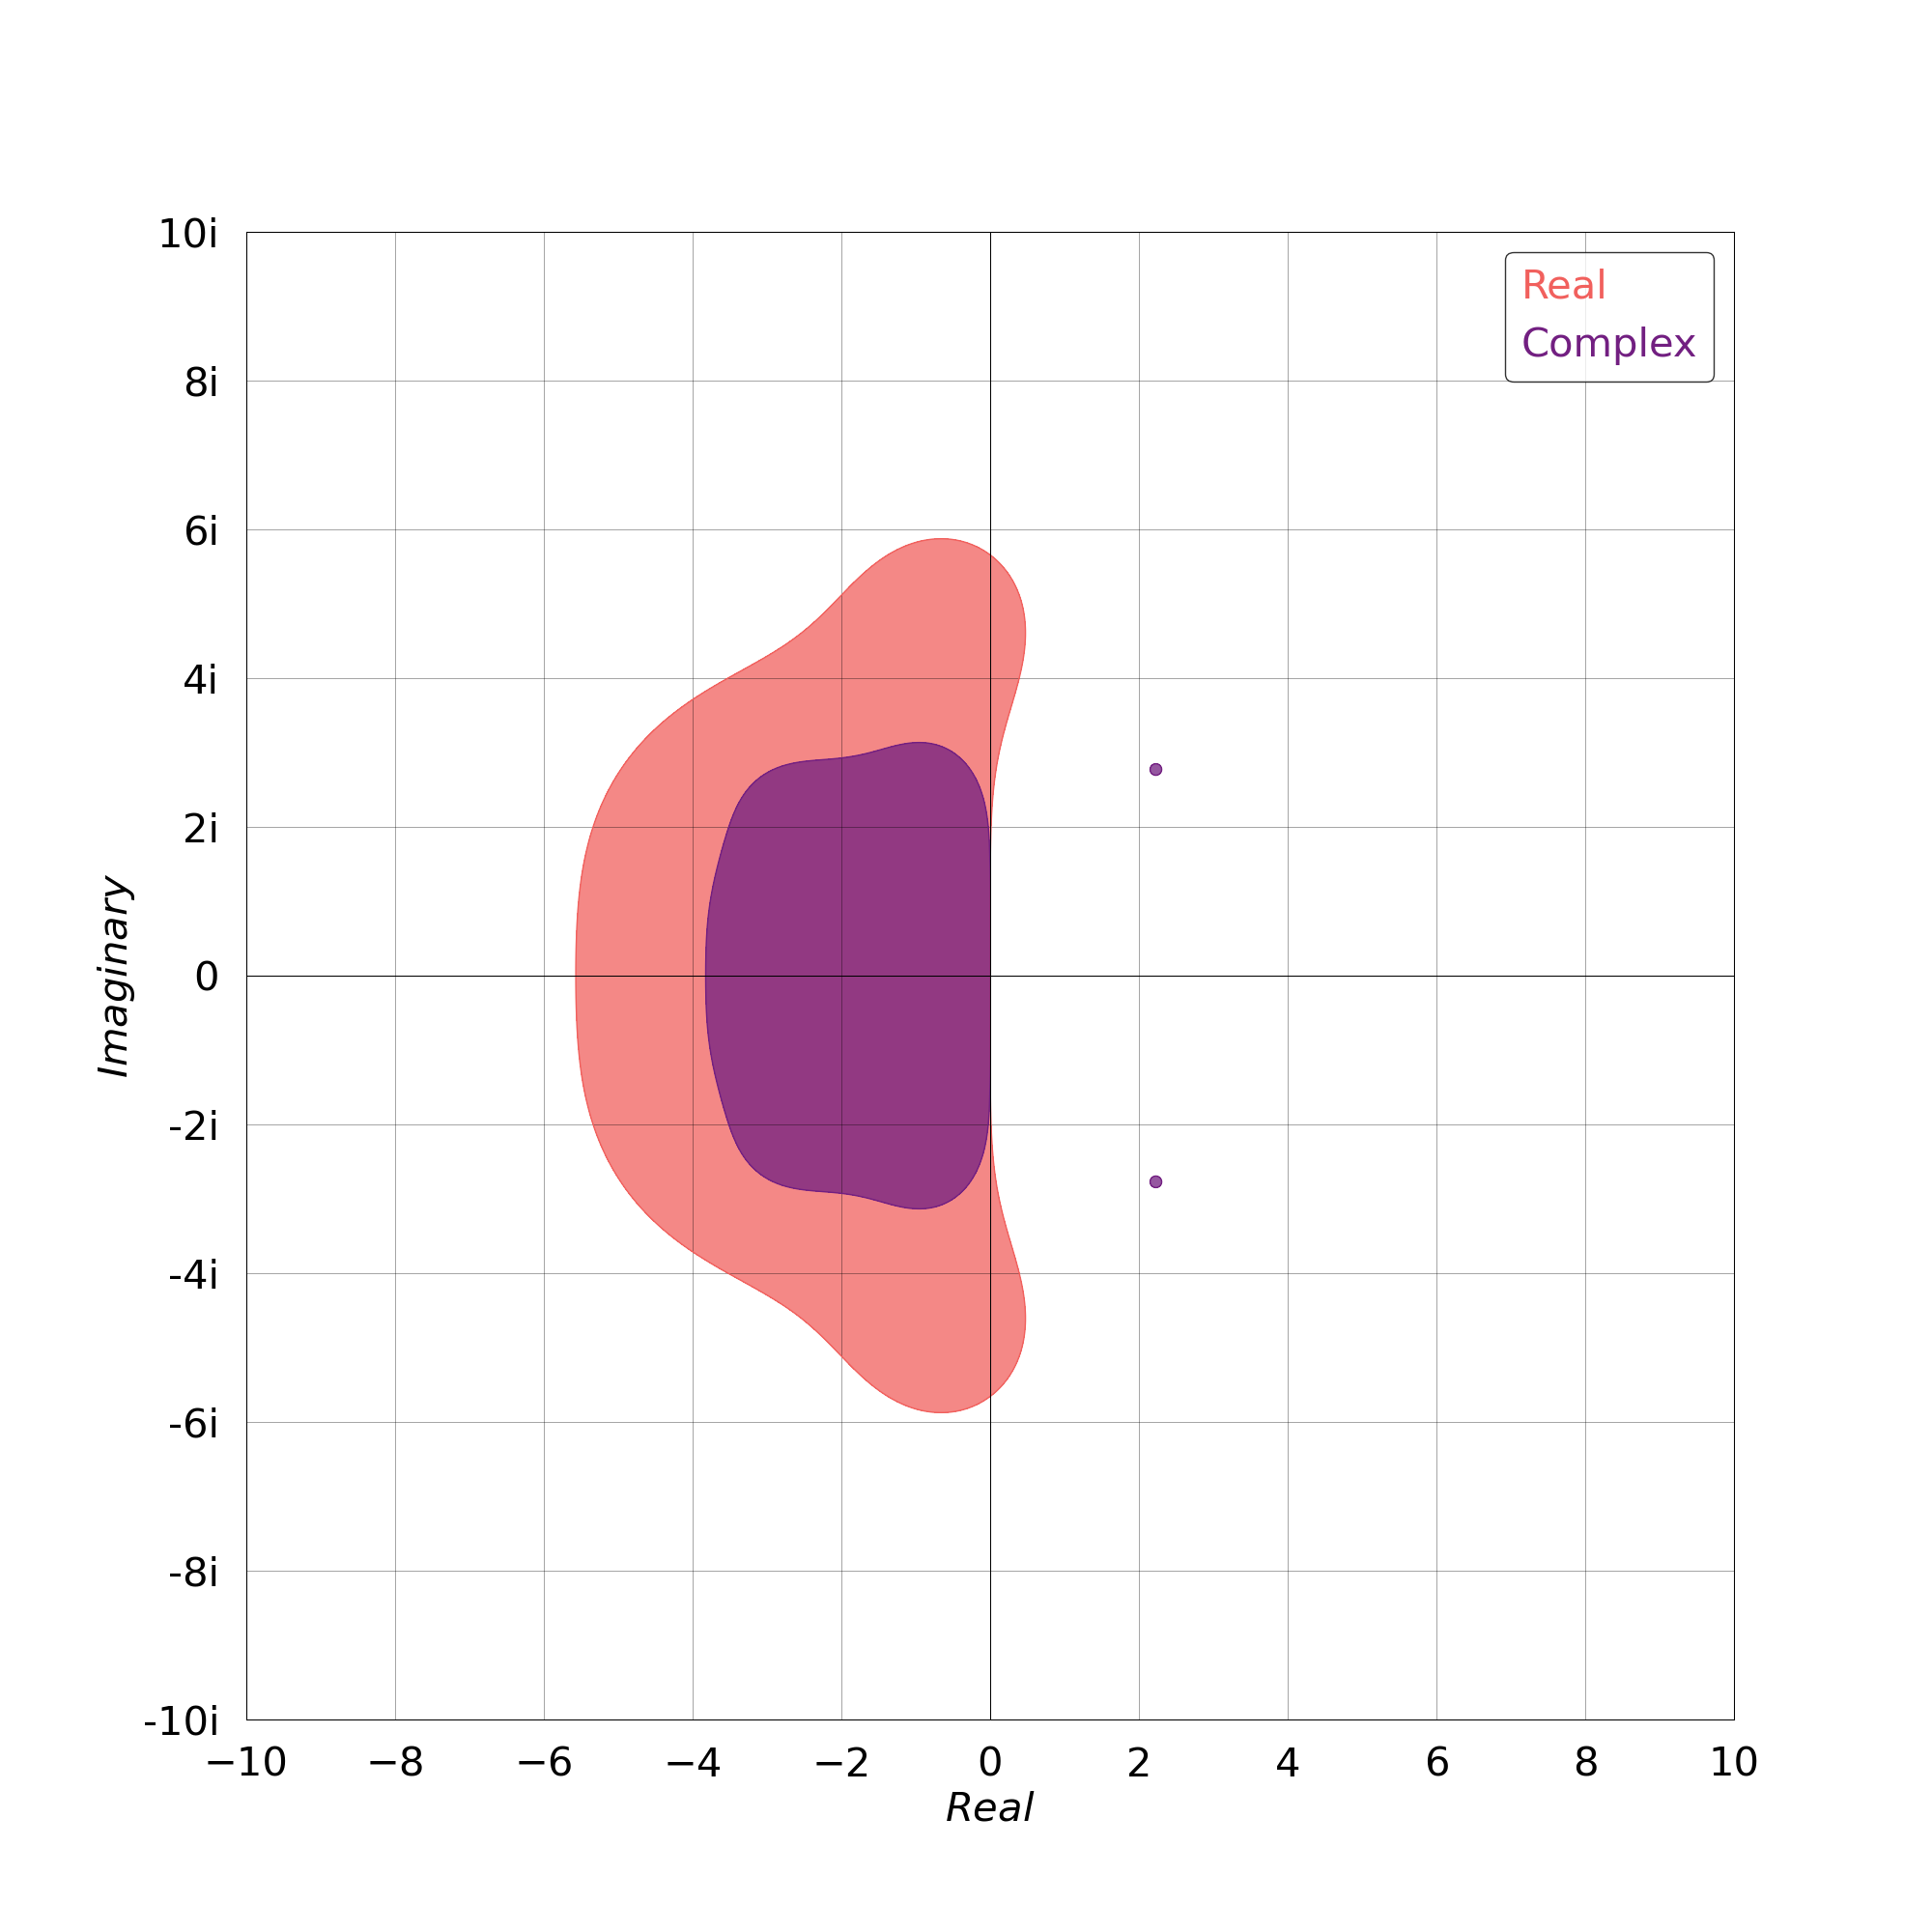
\includegraphics[height=8cm]{Stability Regions/Graphs/Real VS Complex Comparison/Runge-Kutta 4.png}
\columnbreak{}

\textbf{Runge-Kutta 4 2-Step $\bR$}
\begin{flalign*}
    y_{j+1} &= {\bigg(1+z+\frac{z^2}{2}+\frac{z^3}{6}+\frac{z^4}{24}\bigg)}^2 y_j && \\
    y_{j+1} &= \bigg(1+\lh+{(\lh)}^2+\frac{{(\lh)}^3}{6}+\frac{{(\lh)}^4}{24} && \\
            &\quad\,\,\,\,+\frac{{(\lh)}^5}{128}+\frac{5{(\lh)}^6}{4608}+\frac{{(\lh)}^7}{9216}+\frac{{(\lh)}^8}{147456}\bigg) y_j && \\
    \implies &s_{_{\bR}}(\lambda, h) = 1+\lh+{(\lh)}^2+\frac{{(\lh)}^3}{6}+\frac{{(\lh)}^4}{24} && \\
            &\quad\,\,\,\,+\frac{{(\lh)}^5}{128}+\frac{5{(\lh)}^6}{4608}+\frac{{(\lh)}^7}{9216}+\frac{{(\lh)}^8}{147456} &&
\end{flalign*}

\end{multicols}

Computer Calculated Complex - Should probably be checked\\
$1 + \lh + \frac{\lh^2}{2} + \frac{\lh^3}{6} + \frac{\lh^4}{24} + \frac{\lh^5}{128} + \frac{5 \lh^6}{4608} + \frac{\lh^7}{9216} + \frac{\lh^8}{147456} + \frac{b^2 \lh^3}{48} + \frac{b^2 \lh^4}{128} + \frac{b^2 \lh^5}{768} + \frac{b^2 \lh^6}{9216} + \frac{b^4 \lh}{24} - \frac{b^4 \lh^2}{96} + \frac{b^4 \lh^3}{192} + \frac{b^4 \lh^4}{1536} - \frac{b^6}{72} + \frac{b^6 \lh}{144} + \frac{b^6 \lh^2}{576} + \frac{b^8}{576}$

\newpage
\providecommand{\bysame}{\leavevmode\hbox to3em{\hrulefill}\thinspace}
\providecommand{\href}[2]{#2}
\begin{thebibliography}{1}

\bibitem{trefethen_definition}
Llyod N. Trefethen, \emph{{T}he definition of numerical analysis}, Cornell University, 1992.

\bibitem{walking_into_the_complex_domain}
Jithin D. George, Samuel Y. Jung, and Niall M. Mangan, \emph{{W}alking into the complex plane to `order' better time integrators}, \url{https://arxiv.org/abs/2110.04402}, 2021.

\bibitem{next}
Next reference.

\end{thebibliography}
 % bibliography

\end{document}
